\chapter{2019年「数字电路A」\hdu 期末试题}
\date{2020年1月}{郑雪峰，陈龙，盛庆华等}{A0402900}
{未央物理讲师 \href{https://qm.qq.com/q/UPbGudx8cK}{\textbf{Axia}}}
{\qrcode{https://qm.qq.com/q/L3bwJSKAYo}}{HDU 邮电营}
{\qrcode{http://weixin.qq.com/r/mhKYgFTEMQlOrRDj90eI}}{未央学社公众号}
\section{基础题（共24分）}
\begin{exercise}[14]{触发器}
    下图所示是一个由\textbf{下降沿}D触发器构成的A-B触发器.

\vspace{1em}
\begin{minipage}{0.48\textwidth}
\centering
\begin{circuitikz}[scale=0.5]
    % 触发器
    \draw (14,4) node[fill=2号色!10,fill opacity=0.7,flipflop def={t3=CP},flipflop D] (ffD1) {};
    \draw (ffD1.pin 4) --++(0.5,0) node [anchor=west] {$\overline{\text{Q}}$};
    \draw (ffD1.pin 6) --++(0.5,0) node [anchor=west] {Q};
    \draw [anchor=east,thick] (ffD1.bpin 3) to[short,-o,fill=backgroundcolor] (ffD1.bpin 3);% 时钟下降沿有效
    % 门电路
    \draw let \p1=(ffD1.pin 1) in (\x1,\y1) node[nand port] (nand3) at (\x1-2cm,\y1) {};% 与非门3
    \draw let \p1=(nand3.in 1) in (\x1,\y1) node[nand port] (nand1) at (\x1-2cm,\y1+1cm) {};%与非门1
    \draw let \p1=(nand3.in 2) in (\x1,\y1) node[nand port] (nand2) at (\x1-2cm,\y1-1cm) {};%与非门2
    \draw (nand1.in 2)-- ++(-4,0) node [anchor=east] (A) {A};% A口
    \draw let \p1=(nand2.in 1) in (\x1,\y1) node[not port] (notB) at (\x1-2cm,\y1) {};% 非门B
    \draw let \p1=(notB.in),\p2=(nand1.in 2) in (\x1,\y1) (\x2,\y2) (notB.in)--++($(\x2,0)-(\x1,0)-(4,0)$) {} node [anchor=east] {B};% B口
    \draw let \p1=(ffD1.pin 3), \p2=(notB) in (\x1,\y1) (\x2,\y2) node[not port] (notC) at (\x2,\y1) {};% 非门C
    \draw let \p1=(notC.in),\p2=(nand1.in 2) in (\x1,\y1) (\x2,\y2) (notC.in)--++($(\x2,0)-(\x1,0)-(4,0)$) {} node [anchor=east] {CP};% C口
    % 连线
    \draw (notB.out)--(nand2.in 1);% 非门B到与非门2-1口
    \draw (notC.out)--(ffD1.pin 3);% 非门C到时钟口
    \draw (nand1.out)-|(nand3.in 1);% 与非门1到与非门3-1口
    \draw (nand2.out)-|(nand3.in 2);% 与非门1到与非门3-2口
    \draw (nand3.out)--(ffD1.pin 1);
    % 与非门2-2口到触发器Q非端
    \draw (nand1.in 1) -| (5,8);
    \draw (5,8) -| ($(ffD1.pin 4)-(0.1,0)$);
    \draw (ffD1.pin 4) to[short,-*] ($(ffD1.pin 4)-(0.1,0)$);
    % 与非门2-2口到触发器Q端
    \draw (nand2.in 2) -| (5,1);
    \draw (5,1) -| ($(ffD1.pin 6)+(0.2,0)$);
    \draw (ffD1.pin 6) to[short,-*] ($(ffD1.pin 6)+(0.2,0)$);
\end{circuitikz}
\end{minipage}
\hfill
\begin{minipage}{0.48\textwidth}
    \centering
    \begin{tikzpicture}
        \foreach \a in {0,...,5}
        \draw [thick,xshift=\a cm] (0.25,0)--(0.5,0)--(0.5,0.5)--(1,0.5)--(1,0)--(1.25,0);
        \node at (0,0.25) {CP};
        \foreach \b in {0,0.5,...,5.5}
        \draw [densely dashed,xshift=\b cm] (0.5,0.5)--(0.5,-3.2);
        \draw [thick,yshift=-1cm] (0.25,0)--(1.25,0)--(1.25,0.5)--(2.25,0.5)--(2.25,0)--(3.25,0)--(3.25,0.5)--(5.1,0.5)--(5.1,0)--(6.25,0);
        \node [yshift=-1cm] at (0,0.25) {A};
        \draw [thick,yshift=-2cm] (0.25,0)--(1.25,0)--(1.25,0.5)--(2.25,0.5)--(2.25,0)--(3.25,0)--(3.25,0.5)--(4.65,0.5)--(4.65,0)--(4.85,0)--(4.85,0.5)--(5.25,0.5)--(5.25,0)--(6.25,0);
        \node [yshift=-2cm] at (0,0.25) {B};
        \draw [ultra thick,solutioncolor,yshift=-3cm] (0.25,0)--(1.5,0)--(1.5,0.5)--(2.5,0.5)--(2.5,0)--(3.5,0)--(3.5,0.5)--(4.5,0.5)--(4.5,0)--(6.25,0);
        \node [yshift=-3cm] at (0,0.25) {Q};
    \end{tikzpicture}
\end{minipage}
\vspace{1em}

\begin{enumerate}
    \item 写出电路的激励方程和状态方程（5分）.
    \item 电路时上跳沿触发还是下跳沿触发？写出其状态转换真值表或功能特性表（5分）.
    \item 画出图中Q的波形（Q的初始值为$0$）（4分）.
\end{enumerate}
\end{exercise}
\begin{solution}
\begin{enumerate}
    \item 激励方程
    $$D=\overline{\overline{A\overline{Q^n}}\cdot\overline{\overline{B}Q^n}}\xlongequal{\text{De Morgen}}A\overline{Q^n}+\overline{B}Q^n\eqno\point{3}$$

    状态方程
    $$Q^{n+1}=D=A\overline{Q^n}+\overline{B}Q^n\eqno\point{2}$$
    \item 由于CP端口输入通路上有两个非门，所以电路时上升沿触发.\point{1}
\begin{itemize}
    \item 将ABQ所有的可能（从000到111）代入状态方程即可得状态转换表
    \item 将转换表中每一种AB对应的$\text{Q}^n$到$\text{Q}^{n+1}$的变化整理即可得到特性表
\end{itemize}


\vspace{1em}
    \begin{minipage}{0.54\textwidth}

        \centering
        \begin{tabular}{cccc|cccc}
            \toprule
            A & B & $\text{Q}^n$ & $\text{Q}^{n+1}$& A & B & $\text{Q}^n$ & $\text{Q}^{n+1}$\\
            \toprule
            $0$ & $0$ & $0$ & $0$ & $1$ & $0$ & $0$ & $1$\\
            $0$ & $0$ & $1$ & $1$ & $1$ & $0$ & $1$ & $1$\\
            $0$ & $1$ & $0$ & $0$ & $1$ & $1$ & $0$ & $1$\\
            $0$ & $1$ & $1$ & $0$ & $1$ & $1$ & $1$ & $0$\\
            \bottomrule
        \end{tabular}\point{4}
    \end{minipage}
    \hfill
    \begin{minipage}{0.42\textwidth}
        \centering
        \begin{tabular}{cccc|c}
            \toprule
            CP & A & B & $\text{Q}^{n+1}$ & 功能描述\\
            \toprule
            $\uparrow$ & $0$ & $0$ & $0$ & 保持\\
            $\uparrow$ & $0$ & $1$ & $0$ & 复位\\
            $\uparrow$ & $1$ & $0$ & $1$ & 置一\\
            $\uparrow$ & $1$ & $1$ & $\overline{\text{Q}^n}$ & 翻转\\
            \bottomrule
        \end{tabular}\point{4}
    \end{minipage}
\vspace{1em}

    \item 根据特性表即可画出Q的波形.\point{4}
\end{enumerate}
\end{solution}

\begin{exercise}[10]{\texttt{74LS161}}
    \texttt{74LS161}是同步$4$位二进制加法计数器，其逻辑功能表如下.试分析由\texttt{74LS161}组成的时序电路功能.

    \vspace{1em}
\begin{minipage}{0.54\textwidth}
\centering
\begin{tabular}{c|c|c|c|c|llll}
    \toprule
    $\overline{\text{CR}}$ &$\overline{\text{LD}}$ & CTP & CTT & CP & Q3&Q2&Q1&Q0\\
    \toprule
    $0$ & $\times$ & $\times$ & $\times$ & $\times$ & 0&0&0&0\\
    $1$ & $0$ & $\times$ & $\times$ & $\uparrow$ & D3&D2&D1&D0\\
    $1$ & $1$ & $0$ & $\times$ & $\times$ & Q3&Q2&Q1&Q0\\
    $1$ & $1$ & $\times$ & $0$ & $\times$ & Q3&Q2&Q1&Q0\\
    $1$ & $1$ & $1$ & $1$ & $\uparrow$ &加&法&计&数\\
    \bottomrule
\end{tabular}
\end{minipage}
\hfill
\begin{minipage}{0.42\textwidth}
\centering
\begin{circuitikz}[scale=0.5]
    \draw [thick] (0,0) rectangle (10,4);
    \node at (5,2) {\texttt{74LS161}};
    \foreach \a in {2,4,...,8}
    \draw [xshift=\a cm] (0,4)--(0,5);
    \draw (6,5)--++(0,0.5);
    \node [nand port,rotate=-90] (nand1) at (-2,2){};% 与非门
    \draw (6,5.5)-|(nand1.in 2);% Q1到与非门2号口
    \draw (2,5)-|(nand1.in 1);% Q3到与非门2号口
    \draw [anchor=north] (0.625,-1) to[short,-o,fill=backgroundcolor] (0.625,0);
    \draw [anchor=north] (1.875,-1) to[short,-o,fill=backgroundcolor] (1.875,0);
    \foreach \b in {1.25,2.5,...,8}
    \draw [anchor=north,xshift=\b cm] (1.875,-1)--(1.875,0);
    \draw (0.625,-1)-|(nand1.out);% CR到与非门出口
    \draw (0,2)--(-1,2) node [anchor=west,at start] {CO};
    \draw (10,2)--(11,2) node [anchor=east,at start] {CP};
    \node [anchor=north] at (1.875,-1) {$1$} node [anchor=north] at (3.125,-1) {$1$} node [anchor=north] at (4.375,-1) {$1$};
    \node [anchor=north] at (2,4) {$\text{Q}_3$} node [anchor=north] at (4,4) {$\text{Q}_2$} node [anchor=north] at (6,4) {$\text{Q}_1$} node [anchor=north] at (8,4) {$\text{Q}_0$};
    \footnotesize
    \node [anchor=south] at (0.625,0) {$\overline{\text{CR}}$} node [anchor=south] at (1.875,0) {$\overline{\text{LD}}$} node [anchor=south] at (3.125,0) {$\overline{\text{CTP}}$} node [anchor=south] at (4.375,0) {$\overline{\text{CTT}}$} node [anchor=south] at (5.625,0) {$\overline{\text{D3}}$} node [anchor=south] at (6.875,0) {$\overline{\text{D2}}$} node [anchor=south] at (8.125,0) {$\overline{\text{D1}}$} node [anchor=south] at (9.375,0) {$\overline{\text{D0}}$};
\end{circuitikz}
\end{minipage}
\normalsize
\vspace{1em}

\begin{enumerate}
    \item 画出电路的状态转移图.
    \item 说明该电路的逻辑功能.
\end{enumerate}
\end{exercise}
\begin{solution}
    \begin{enumerate}
        \item 根据功能表和电路图可知，当$\text{Q3Q2Q1Q0}=1010$时电路清零，其余情况均在加法计数.所以状态转移图为\point{6}
        
        \vspace{1em}
        \centering
        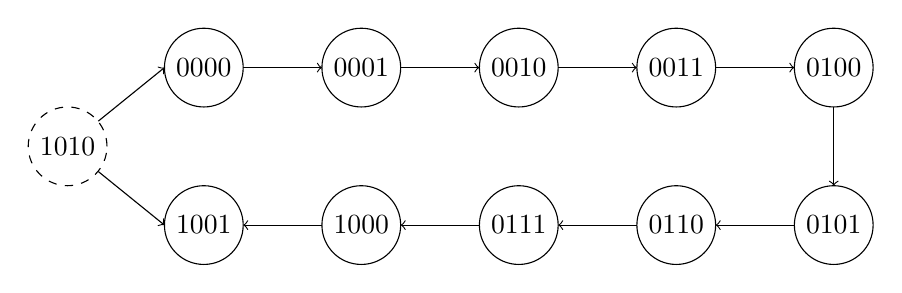
\begin{tikzpicture}
            \foreach \a in {0,2,...,8}
            \foreach \b in {0,-2}
            \draw [xshift=\a cm,yshift=\b cm] (0,0) circle (0.5);
            \foreach \c in {0,2,4,6}
            \draw [xshift=\c cm,->] (0.5,0)--(1.5,0);
            \foreach \d in {0,2,4,6}
            \draw [xshift=\d cm,<-] (0.5,-2)--(1.5,-2);
            \draw [->] (8,-0.5)--(8,-1.5);
            \draw [dashed] (-1.73,-1) circle (0.5);
            \draw [->] (-1.34,-0.68)--(-0.5,0);
            \draw [->] (-1.34,-1.32)--(-0.5,-2);
            \node at (0,0) {0000} node at (2,0) {0001} node at (4,0) {0010} node at (6,0) {0011} node at (8,0) {0100} node at (8,-2) {0101} node at (6,-2) {0110} node at (4,-2) {0111} node at (2,-2) {1000} node at (0,-2) {1001} node at (-1.73,-1) {1010};
        \end{tikzpicture}
        \item 由电路的状态转移图可知其“满十进一”，所以其功能为10进制的加法计数器.\point{4}
    \end{enumerate}
\end{solution}

\section{设计题（共36分）}
\begin{exercise}[16]{逻辑抽象，\texttt{74LS138}}
    某机床由A、B、C三台电动机拖动，根据加工要求为
    \begin{itemize}
        \item A机必须开机运行
        \item 如开B机，则必须开C机
        \item A机运行后，C机器
        \item 也可以开机运行
    \end{itemize}
    满足上述要求时，指示灯亮，否则只是灯熄灭.设开机信号为$1$，指示灯亮为$1$.
\begin{enumerate}
    \item 进行逻辑抽象和逻辑定义.
    \item 设计出电路的真值表.
    \item 使用\texttt{74LS138}译码器实现该电路，并画出电路图.
\end{enumerate}
\end{exercise}
\begin{solution}
\begin{enumerate}
    \item A、B、C三台电机分别用A、B、C表示，$1$表示开机，$0$表示关机.\point{2}
    
    指示灯用F表示，$1$表示灯亮，$0$表示灯灭.\point{2}
    
    \begin{multicols}{2}
\item 真值表为\point{7}

    \vspace{1em}
    \centering
    \begin{tabular}{cccc|cccc}
        \toprule
        A & B & C & F & A & B & C & F\\
        \toprule
        0 & 0 & 0 & 0 & 1 & 0 & 0 & 1\\
        0 & 0 & 1 & 0 & 1 & 0 & 1 & 1\\
        0 & 1 & 0 & 0 & 1 & 1 & 0 & 0\\
        0 & 1 & 1 & 0 & 1 & 1 & 1 & 1\\
        \bottomrule
    \end{tabular}

    \item 由真值表得$\text{F}=m_4+m_5+m_7=\overline{\overline{\text{Y}}_4\overline{\text{Y}}_5\overline{\text{Y}}_7}$.由于A为高位，所以A连$\text{A}_2$端，B连$\text{A}_1$端，C连$\text{A}_0$端.\point{5}
    
    \centering
\begin{circuitikz}[scale=0.5]
    \draw [thick] (0,0) rectangle (10,4);
    \node at (5,2) {\texttt{74LS138}};
    \foreach \a in {1.25,2.5,3.75,6.25,7.5,8.75}
    \draw [xshift=\a cm] (0,4)--(0,4.5);
    
    \foreach \b in {0,1.25,2.5,3.75,5,6.25,7.5,8.75}
    \draw [anchor=north,xshift=\b cm] (0.625,-0.6) to[short,-o,fill=backgroundcolor] (0.625,0);% Y圈

    \node [anchor=north] at (1.25,4) {$\text{S}_1$} node [anchor=north] at (2.5,4) {$\overline{\text{S}}_2$} node [anchor=north] at (3.75,4) {$\overline{\text{S}}_3$} node [anchor=north] at (6.25,4) {$\text{A}_2$} node [anchor=north] at (7.5,4) {$\text{A}_1$} node [anchor=north] at (8.75,4) {$\text{A}_0$};

    \node [anchor=south] at (1.25,4.5) {$1$} node [anchor=south] at (2.5,4.5) {$0$} node [anchor=south] at (3.75,4.5) {$0$} node [anchor=south] at (6.25,4.5) {A} node [anchor=south] at (7.5,4.5) {B} node [anchor=south] at (8.75,4.5) {C};

    \node [anchor=south] at (0.625,0) {$\overline{\text{Y}}_0$} node [anchor=south] at (1.875,0) {$\overline{\text{Y}}_1$} node [anchor=south] at (3.125,0) {$\overline{\text{Y}}_2$} node [anchor=south] at (4.375,0) {$\overline{\text{Y}}_3$} node [anchor=south] at (5.625,0) {$\overline{\text{Y}}_4$} node [anchor=south] at (6.875,0) {$\overline{\text{Y}}_5$} node [anchor=south] at (8.125,0) {$\overline{\text{Y}}_6$} node [anchor=south] at (9.375,0) {$\overline{\text{Y}}_7$};

    \draw (5.625,-0.6)--(5.625,-1.2);
    \draw (6.875,-0.6)--(6.875,-1.0);
    \draw (9.375,-0.6)--(9.375,-0.8);

    \node [nand port,number inputs=3,rotate=90] (nand1) at (12,2) {};
    \draw (nand1.in 1)--++(0,-1.5)-|(9.375,-0.8);
    \draw (nand1.in 2)--++(0,-1.7)-|(6.875,-1.0);
    \draw (nand1.in 3)--++(0,-1.9)-|(5.625,-1.2);
    \draw (nand1.out)--++(0,0.5) node [anchor=south] {F};
\end{circuitikz}
    \end{multicols}
\end{enumerate}
\end{solution}
\begin{note}
\begin{center}  
    \begin{tabular}{c|c|c}
        \toprule
        \multicolumn{1}{c|}{\multirow{2}{*}{函数}} & \multicolumn{2}{c}{译码器} \\
        \cmidrule{2-3}
        & \multicolumn{1}{c|}{高电平译码输出有效} & \multicolumn{1}{c}{低电平译码输出有效} \\
        \toprule
        译码输出端 & $\text{Y}_i=m_i=\overline{M_i}$ & $\text{Y}_i=M_i=\overline{m_i}$ \\
        最小项之和 & 外加或门 & 外加与非门 \\
        最大项之和 & 外加或非门 & 外加与门 \\
        \bottomrule
    \end{tabular}
\end{center}
\end{note}

\begin{exercise}[20]{逻辑抽象，D触发器}
    步进电机的控制绕组有$4$种通电状态，分别为A、B、C、D.它的旋转增量为$1.8^{\circ}$，旋转$200$步构成一周.电机X正转时，按照$\text{A}\to\text{B}\to\text{C}\to\text{D}\to\text{A}$的通电次序；电机X反转时，按照$\text{A}\to\text{D}\to\text{C}\to\text{B}\to\text{A}$的通电次序.如果控制绕组的通电次序用计数器控制实现（计数器的某一状态对应某一绕组的通电状态），电机每转一圈在D通电时，指示灯亮.
\begin{enumerate}
    \item 进行逻辑抽象和逻辑定义，设计原始状态图、原始状态表（6分）.
    \item 列出状态转换真值表，求出方程组（10分）.
    \item 完成设计，并用D触发器设计电路图（4分）.
\end{enumerate}
\end{exercise}
\begin{solution}
    \centering
    \includegraphics[width=\textwidth]{19-4-4.jpg}
\end{solution}